%%
%% Copyright 2007, 2008, 2009 Elsevier Ltd
%%
%% This file is part of the 'Elsarticle Bundle'.
%% ---------------------------------------------
%%
%% It may be distributed under the conditions of the LaTeX Project Public
%% License, either version 1.2 of this license or (at your option) any
%% later version.  The latest version of this license is in
%%    http://www.latex-project.org/lppl.txt
%% and version 1.2 or later is part of all distributions of LaTeX
%% version 1999/12/01 or later.
%%
%% The list of all files belonging to the 'Elsarticle Bundle' is
%% given in the file `manifest.txt'.
%%

%% Template article for Elsevier's document class `elsarticle'
%% with numbered style bibliographic references
%% SP 2008/03/01
%%
%%
%%
%% $Id: elsarticle-template-num.tex 4 2009-10-24 08:22:58Z rishi $
%%
%%
\documentclass[preprint,12pt]{elsarticle}

%% Use the option review to obtain double line spacing
%% \documentclass[preprint,review,12pt]{elsarticle}

%% Use the options 1p,twocolumn; 3p; 3p,twocolumn; 5p; or 5p,twocolumn
%% for a journal layout:
%% \documentclass[final,1p,times]{elsarticle}
%% \documentclass[final,1p,times,twocolumn]{elsarticle}
%% \documentclass[final,3p,times]{elsarticle}
%% \documentclass[final,3p,times,twocolumn]{elsarticle}
%% \documentclass[final,5p,times]{elsarticle}
%% \documentclass[final,5p,times,twocolumn]{elsarticle}

%% if you use PostScript figures in your article
%% use the graphics package for simple commands
%% \usepackage{graphics}
%% or use the graphicx package for more complicated commands
%% \usepackage{graphicx}
%% or use the epsfig package if you prefer to use the old commands
%% \usepackage{epsfig}

%% The amssymb package provides various useful mathematical symbols
\usepackage{amssymb}
%% The amsthm package provides extended theorem environments
%% \usepackage{amsthm}
\usepackage[portuguese]{babel}
\usepackage[utf8]{inputenc}

\graphicspath{{figure/}}
\usepackage{amsmath} 
\usepackage{graphicx} 
\usepackage{epstopdf}
\usepackage{subfigure}
\usepackage{float}
\usepackage{listings}


\usepackage{multirow}
\usepackage{booktabs}
\usepackage[table,xcdraw]{xcolor}
\usepackage[numbered, framed]{mcode}
\usepackage[colorinlistoftodos]{todonotes}
%% The lineno packages adds line numbers. Start line numbering with
%% \begin{linenumbers}, end it with \end{linenumbers}. Or switch it on
%% for the whole article with \linenumbers after \end{frontmatter}.
%% \usepackage{lineno}

%% natbib.sty is loaded by default. However, natbib options can be
%% provided with \biboptions{...} command. Following options are
%% valid:

%%   round  -  round parentheses are used (default)
%%   square -  square brackets are used   [option]
%%   curly  -  curly braces are used      {option}
%%   angle  -  angle brackets are used    <option>
%%   semicolon  -  multiple citations separated by semi-colon
%%   colon  - same as semicolon, an earlier confusion
%%   comma  -  separated by comma
%%   numbers-  selects numerical citations
%%   super  -  numerical citations as superscripts
%%   sort   -  sorts multiple citations according to order in ref. list
%%   sort&compress   -  like sort, but also compresses numerical citations
%%   compress - compresses without sorting
%%
%% \biboptions{comma,round}

% \biboptions{}


\journal{...}

\begin{document}
	
	\begin{frontmatter}
		
		%% Title, authors and addresses
		
		%% use the tnoteref command within \title for footnotes;
		%% use the tnotetext command for the associated footnote;
		%% use the fnref command within \author or \address for footnotes;
		%% use the fntext command for the associated footnote;
		%% use the corref command within \author for corresponding author footnotes;
		%% use the cortext command for the associated footnote;
		%% use the ead command for the email address,
		%% and the form \ead[url] for the home page:
		%%
		%% \title{Title\tnoteref{label1}}
		%% \tnotetext[label1]{}
		%% \author{Name\corref{cor1}\fnref{label2}}
		%% \ead{email address}
		%% \ead[url]{home page}
		%% \fntext[label2]{}
		%% \cortext[cor1]{}
		%% \address{Address\fnref{label3}}
		%% \fntext[label3]{}

\title{Implementação da Janela de Parzen utilizando MATLAB}

%% use optional labels to link authors explicitly to addresses:
%% \author[label1,label2]{<author name>}
%% \address[label1]{<address>}
%% \address[label2]{<address>}

{\author[label1]{Gustavo Siebra Lopes}

\address[label1]{Programa de Pós-Graduação em Ciências da Computação, Instituto Federal do Ceará, Fortaleza, CE, Brazil. Email: gustavosiebra@gmail.com}}

\begin{abstract}
Esse trabalho é para compor a nota na disciplina de Aprendizagem de Máquina. Consiste na implementação do código para diferentes bases e segmentação de imagens usando MATLAB, contém um breve relatório sobre as técnicas de reconhecimento de padrão utilizada e seus resultados.
\end{abstract}

\begin{keyword}
%% keywords here, in the form: keyword \sep keyword
Reconhecimento de Padrões, Segmentação, Janela de Parzen, Matlab.
%% MSC codes here, in the form: \MSC code \sep code
%% or \MSC[2008] code \sep code (2000 is the default)

\end{keyword}

\end{frontmatter}

%%
%% Start line numbering here if you want
%%
% \linenumbers

%% main text
%\section{}
%\label{}

\section{Preparação da base}

As bases utilizada nesse relatório estão disponibilizadas na UCI Machine Learning Repository. \citep{UCI152015}

\subsection{Base de dados da Flor de Íris}

Nessa base são definidas 3 classes (Íris Setosa, Íris Versicolor, Íris Virgínica) e 4 parâmetros por classe (comprimento e largura da sépala e pétala). A base possui 150 padrões diferentes de Iris dividido em 50 para cada classe.

\subsubsection{Análise das características}
\label{sec:examples}

Na figura \ref{fig:featuresIris} é apresentada a matriz de características. Essa matriz consiste de gráficos formados pelos pares de características combinadas.


\begin{figure}[H]
	\centering
	
	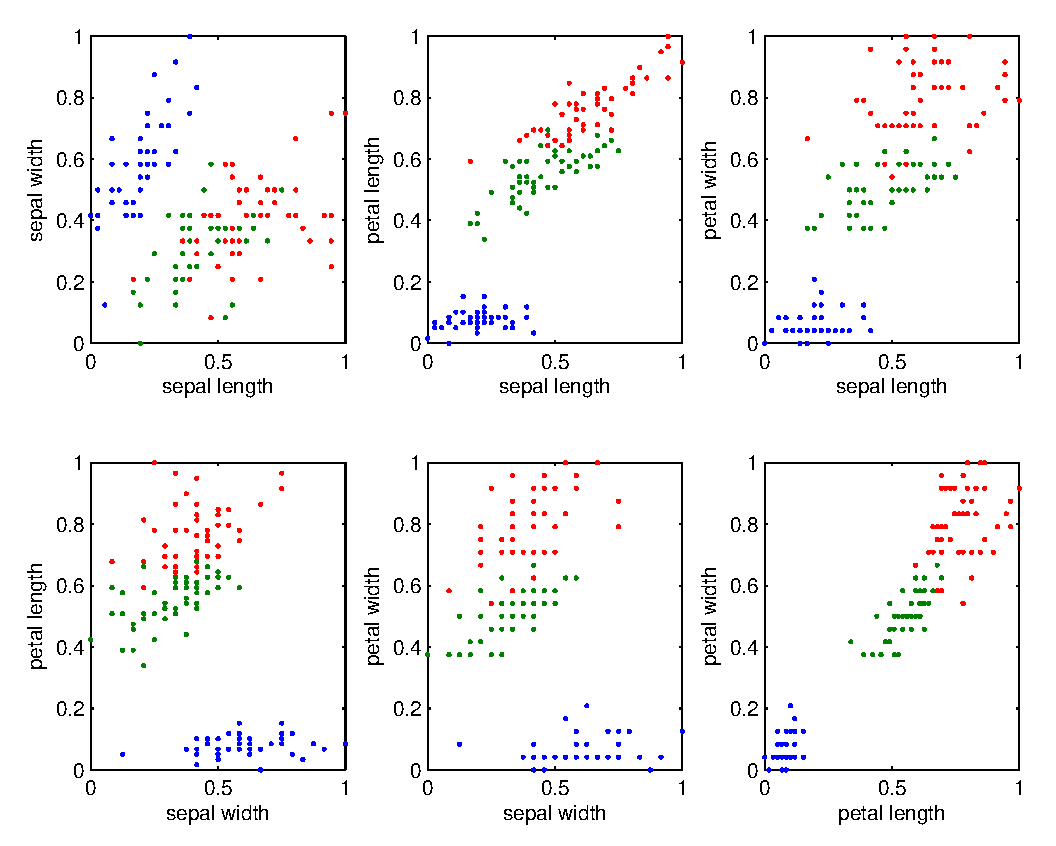
\includegraphics[height=9cm]{figure/myfig.eps}
	
	
	\caption{Matriz de características.}
	\label{fig:featuresIris}
\end{figure}

Podemos perceber que a classe setosa pode facilmente ser separada das outras utilizando a largura ou o comprimento da pétala como variável, já para as duas outras características essa separação não é tão simples, perceba a sobreposição dos histogramas em todos os atributos bem como a mistura das classes nos gráficos de dispersão.

\subsection{Base de dados da Dermatologia}

Esta base de dados contém 34 atributos, 33 dos quais são valorizados linear e um deles é nominal. O diagnóstico diferencial das doenças eritêmato-escamosas é um problema real em dermatologia. Todos eles compartilham as características clínicas de eritema e descamação, com poucas diferenças. As doenças deste grupo são a psoríase, dermatite seborreica, líquen plano, pitiríase rósea, dermatite crônica, e pitiríase rubra pilar. Geralmente é necessário para o diagnóstico de uma biópsia, mas infelizmente essas doenças compartilham muitas características histopatológicas. Uma outra dificuldade para o diagnóstico diferencial é uma doença que pode apresentar as características de uma outra doença na fase inicial e pode ter as características específicas nas fases seguintes. Os pacientes foram avaliados clinicamente primeiro com 12 recursos. Depois disso, amostras de pele foram levados para a avaliação de 22 características histopatológicas. Os valores das características histopatológicas são determinadas por uma análise das amostras sob um microscópio.

No conjunto de dados construída para este domínio, o recurso história familiar tem o valor 1, se qualquer uma destas doenças tem sido observado na família, e 0, caso contrário. A característica idade representa simplesmente a idade do paciente. Cada outro recurso (clínico e histopatológico) foi dado um grau na escala de 0 a 3. Aqui, 0 indica que o recurso não estava presente, 3 indica a maior quantidade possível, e 1, 2 indicam os valores intermediários relativos.

\section{Janela de Parzen}

Em estatística, a estimativa de densidade \textit{Kernel} (EDK) é uma forma não-paramétrica para estimar a função de densidade de probabilidade de uma variável aleatória. Estimação da densidade \textit{Kernel} é um problema fundamental de suavização de dados onde inferências sobre a população são feitas, com base numa amostra de dados finita.

Seja ($x_1$, $x_2$, $\dots$, $x_n$) independentes e amostras identicamente distribuídos retirada de alguma distribuição com uma densidade desconhecida $f$. Estamos interessados em estimar a forma desta função $f$. O estimador de densidade de \textit{kernel} é:

\begin{align}
\text {$f _h$(x) = ($\dfrac{1}{n}$)$\sum_{i=1}^{n}$$K_h$(x - $x_i$) = ($\dfrac{1}{nh}$)$\sum_{i=1}^{n}$K($\dfrac{x - x_i}{h}$)},
\end{align}

onde \textbf{K} (•) é o núcleo - uma função não-negativa que integra a um e tem média zero - e \textbf{h} $>$ 0 é um parâmetro de suavização chamado largura de banda. Um núcleo com índice \textbf{h} é chamado núcleo dimensionado e definido como:

\begin{align}
\text {$K_h$(x) = ($\dfrac{1}{h}$)  $\times$  K($\dfrac{x}{h}$)},
\end{align}

Intuitivamente se quer escolher \textbf{h} tão pequeno quanto os dados permitem, no entanto, há sempre um \textit{trade-off} entre o bias do estimador e sua variância.

As funções de \textit{kernel} que podem ser usadas são: uniforme, triangular,\textit{ biweight, triweight, Epanechnikov}, normais, e outros. O \textit{kernel Epanechnikov} é o ideal em um sentido erro médio quadrado, \citep{Epanechnikov1969} embora a perda de eficiência seja pequena para os \textit{kernels} listadas anteriormente, \citep{Wand1995}, devido às suas propriedades matemáticas convenientes, o \textit{kernel} normal é muitas vezes usado K(x) = $\phi$(x) , onde $\phi$ é o padrão normal da função de densidade.

\section{Algoritmo}

A base foi dividida usando o modelo \textit{holdout}. Este método consiste em dividir o conjunto total de dados em dois subconjuntos mutuamente exclusivos, um para treinamento (estimação dos parâmetros) e outro para teste (validação). O conjunto de dados pode ser separado em quantidades iguais ou não. Uma proporção muito comum é considerar 2/3 dos dados para treinamento e o 1/3 restante para teste. \citep{Kohavi1995}

Após o carregamento da base foi realizado a normalização dos dados separadamente para cada atributo. Identificando o mínimo e o máximo que foram normalizados na faixa [0,1].

O algoritmo tem como objetivo calcular a probabilidade que uma amostra desconhecida pertença a cada uma das classes possíveis, ou seja, predizer a classe mais provável. Este tipo de predição é chamada de classificação estatística, pois é completamente baseada em probabilidades. 

Esse algoritmo requer um conjunto de dados prévio que já esteja classificado, ou seja, um conjunto que já estejam separadas em classes (ou \textit{clusters}). Baseado neste conjunto de dados prévio, que também é chamado de conjunto de treinamento, o algoritmo recebe como entrada uma nova amostra desconhecida, ou seja, que não possui classificação, e retorna como saída a classe mais provável para esta amostra de acordo com cálculos probabilísticos. O algoritmo deve seguir os seguintes passo:\\


\textbf{Passo 01}: Cálculos das probabilidades das classes.\\

Neste passo, cada classe do conjunto de treinamento possui sua probabilidade calculada. O cálculo é feito dividindo-se o número de instâncias de determinada classe pelo número total de instâncias do conjunto de treinamento.\\

\textbf{Passo 02}: Cálculo das probabilidades da amostra desconhecida.\\

Agora, o valor de cada atributo da amostra desconhecida possui sua probabilidade calculada para cada possível classe. Este passo é onde o processamento mais 'pesado' do algoritmo ocorre, pois, dependendo do número de atributos, classes e instâncias do conjunto de treinamento, é possível que muitos cálculos sejam necessários para se obter as probabilidades.

É importante notar que este cálculo depende inteiramente dos valores dos atributos da amostra desconhecida, ou seja, da amostra que se deseja prever a classes. Supondo que existam k classes no conjunto de testes e m atributos conjunto de testes será necessário calcular k x m probabilidades.\\

\textbf{Passo 03}: Calcular a probabilidades da amostra desconhecida.\\

Neste passo, as probabilidades calculadas para os valores da amostra desconhecida de uma mesma classe são multiplicadas. Em seguida, o valor obtido é multiplicado pela probabilidade da classe calculada no Passo 01.

Com as probabilidades de cada classe calculadas, verifica-se qual é a classe que possui maior probabilidade para a amostra desconhecida. Com isso, o algoritmo termina retornando a classe que possui maior probabilidade de conter a amostra desconhecida.


\section{Resultados}

\subsection{Segmentação}

Em visão computacional, segmentação se refere ao processo de dividir uma imagem digital em múltiplas regiões (conjunto de \textit{pixels}) ou objetos, com o objetivo de simplificar e/ou mudar a representação de uma imagem para facilitar a sua análise. Segmentação de imagens é tipicamente usada para localizar objetos e formas (linhas, curvas, etc) em imagens.

O resultado da segmentação de imagens é um conjunto de regiões/objetos. Com o resultado, cada um dos \textit{pixels} em uma mesma região é similar com referência a alguma característica ou propriedade computacional, tais como cor, intensidade, textura ou continuidade. Regiões adjacentes devem possuir diferenças significativas com respeito a mesma característica(s). Esse trabalho a segmentação é feita pela extração das características das cores RGB para o tamanho de janela igual a 3.


\begin{figure}[H]
	\centering
	
	\subfigure[Imagem Original]{ \includegraphics[width=0.4\textwidth]{figure/flagJapan.jpg}}
	\subfigure[Imagem Segmentada]{ \includegraphics[width=0.3\textwidth]{figure/segmentacaoJapao.eps}}
	
	\caption{Resultado da Segmentação da bandeira do Japão.}
	\label{fig:flagJapan}
\end{figure}

\begin{figure}[H]
	\centering
	
	\subfigure[Imagem Original]{ \includegraphics[width=0.4\textwidth]{figure/flagEUA1.jpg}}
	\subfigure[Imagem Segmentada]{ \includegraphics[width=0.3\textwidth]{figure/segmentacaoEUA.eps}}
	
	\caption{Resultado da Segmentação da bandeira dos EUA.}
	\label{fig:flagEUA}
\end{figure}

\begin{figure}[H]
	\centering
	
	\subfigure[Imagem Original]{ \includegraphics[width=0.4\textwidth]{figure/flagFrance.jpg}}
	\subfigure[Imagem Segmentada]{ \includegraphics[width=0.3\textwidth]{figure/segmentacaoFrance.eps}}
	
	\caption{Resultado da Segmentação da bandeira da França.}
	\label{fig:flagFrancen}
\end{figure}


\subsection{Acurácia}

Acurácia é a proporção de acertos, ou seja, o total de verdadeiramente positivos e verdadeiramente negativos, em relação a amostra estudada. O resultado da acurácia foi obtido através de 30 iterações para o tamanho da janela com valor de 0.5, 1, 1.5 e 2. Percebemos nas Figuras \ref{fig:accIris} e \ref{fig:accDerme} que quanto maior for o valor da janela menor será a taxa de acurácia.

\begin{figure}[H]
	\centering
	
	\subfigure[h = 0,5]{ 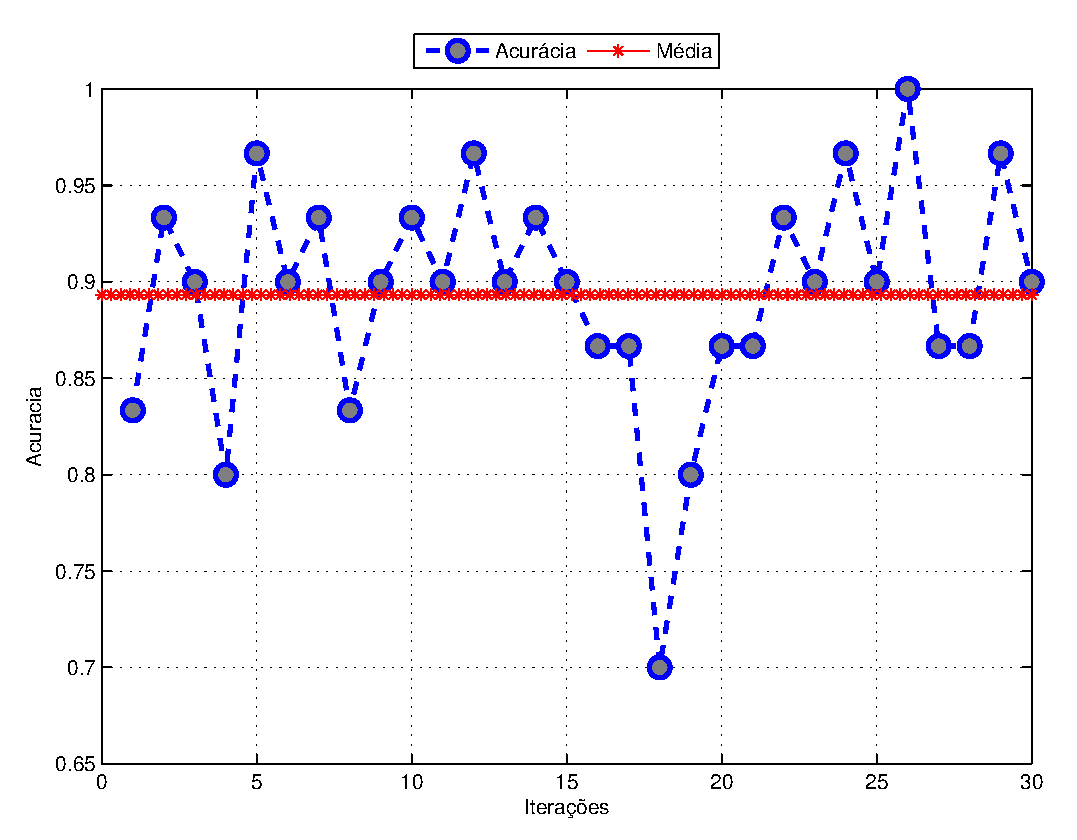
\includegraphics[width=0.4\textwidth]{figure/parzen_h_05.eps}}
	\subfigure[h = 1]{ 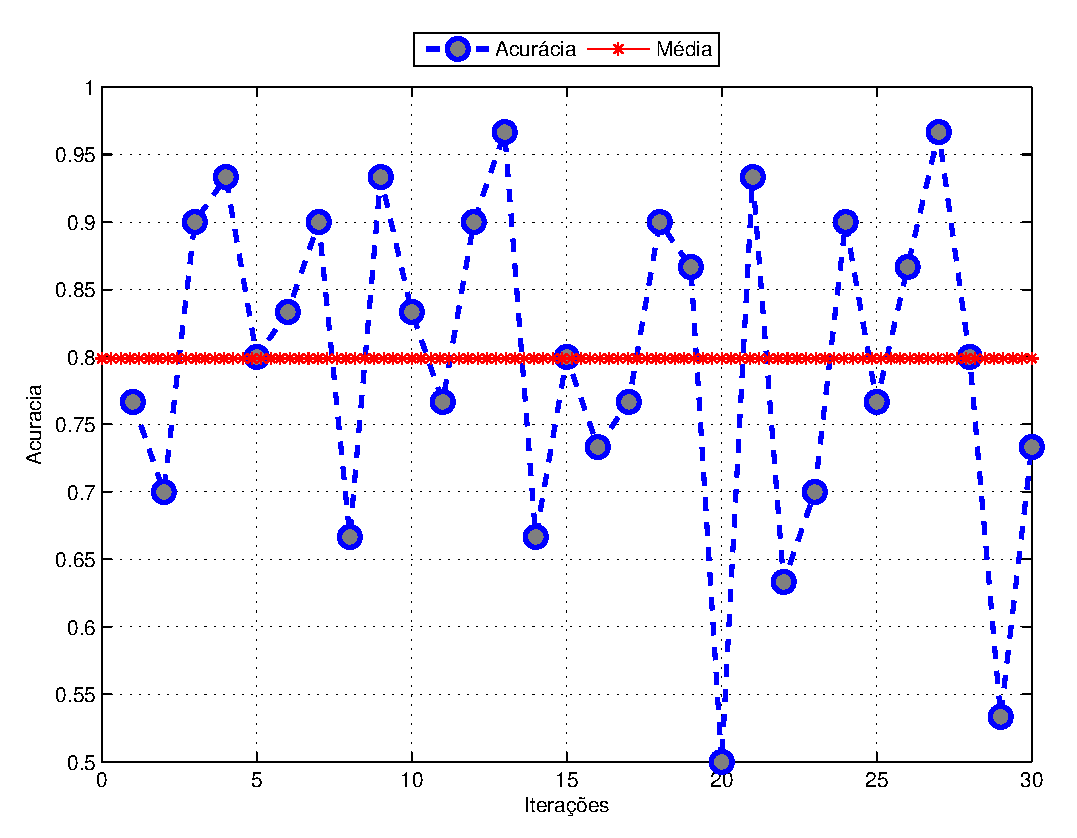
\includegraphics[width=0.4\textwidth]{figure/parzen_h_1.eps}}
	\subfigure[h = 1,5]{ 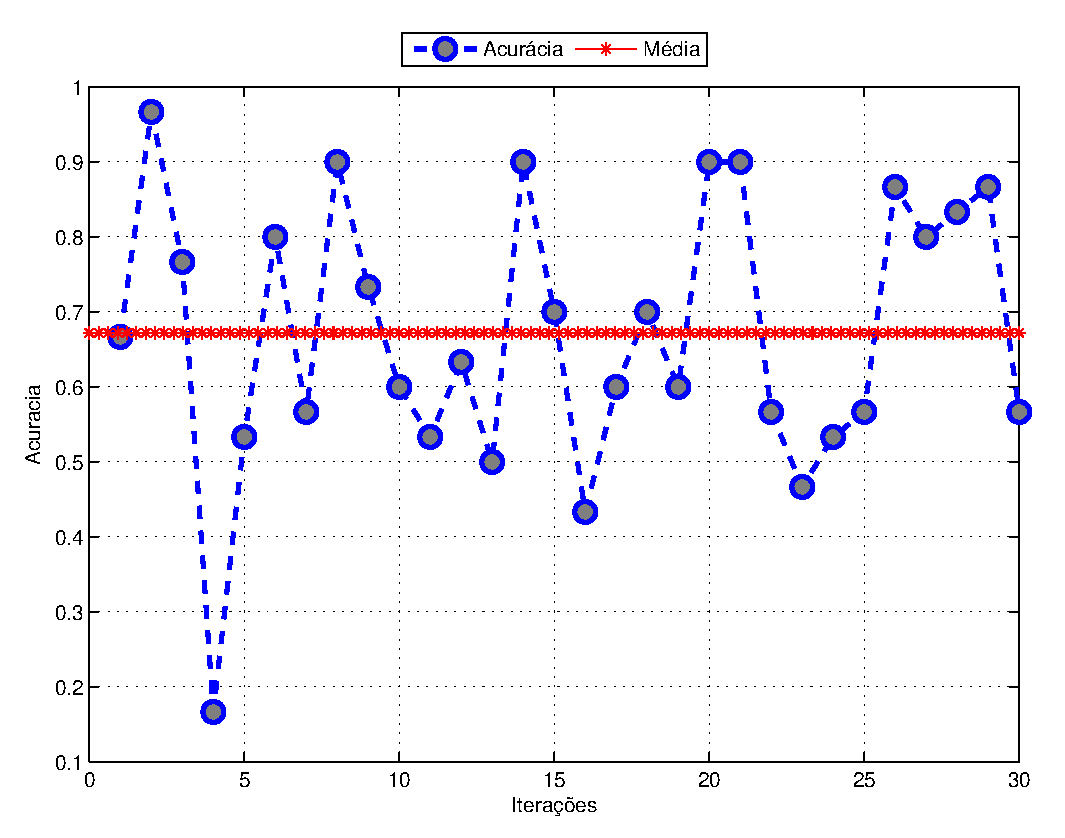
\includegraphics[width=0.4\textwidth]{figure/parzen_h_15.eps}}
	\subfigure[h = 2]{ 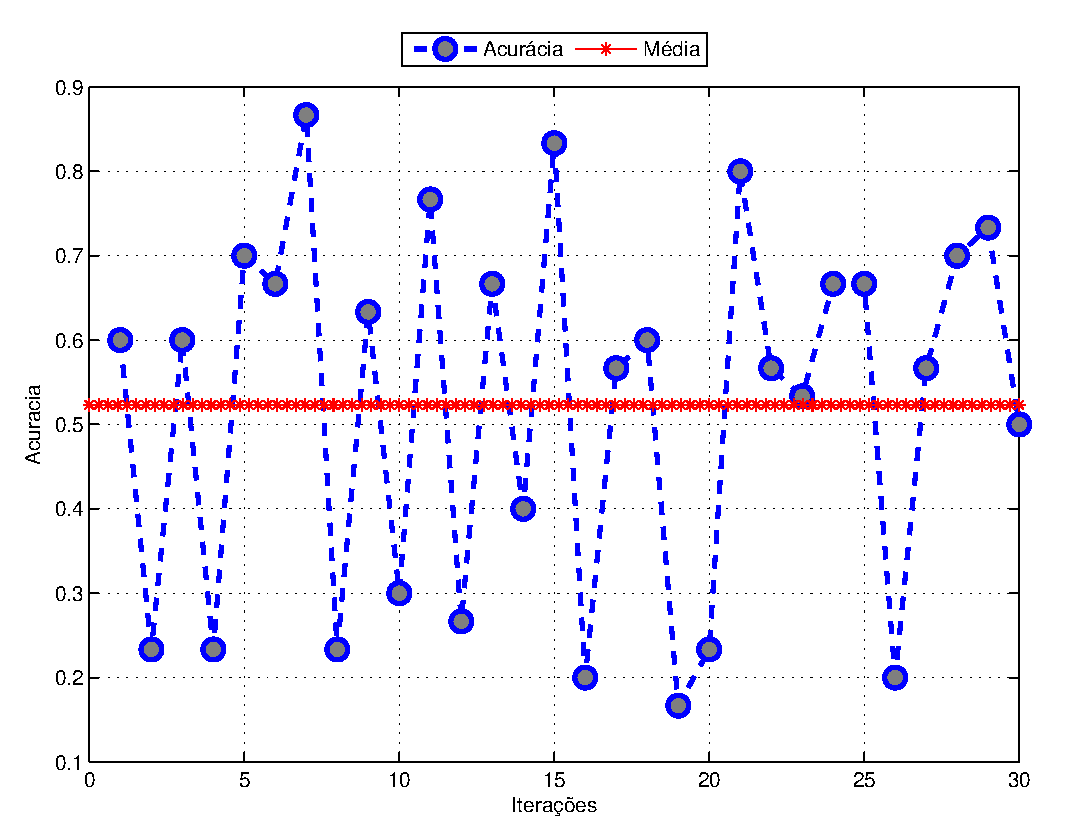
\includegraphics[width=0.4\textwidth]{figure/parzen_h_2.eps}}
	
	\caption{Resultados da Acurácia para flor da Íris.}
	\label{fig:accIris}
\end{figure}

\begin{figure}[H]
	\centering
	
	\subfigure[h = 0,5]{ 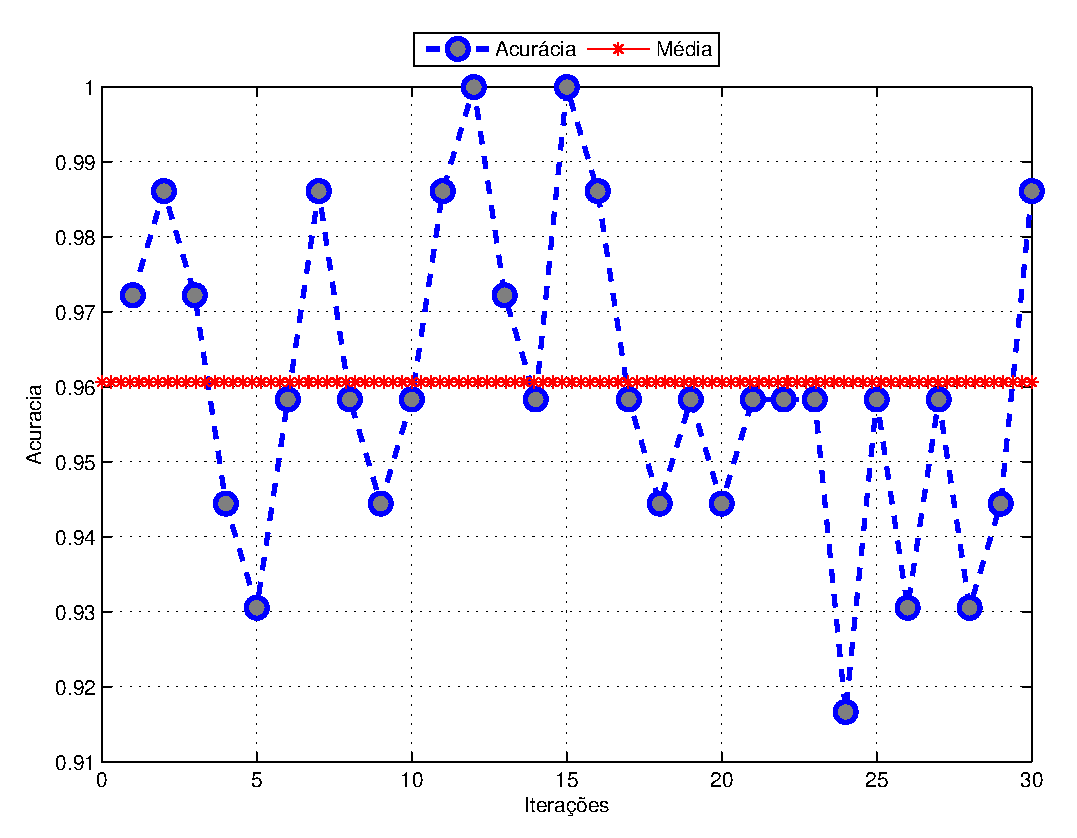
\includegraphics[width=0.4\textwidth]{figure/derme_parzen_h_05.eps}}
	\subfigure[h = 1]{ 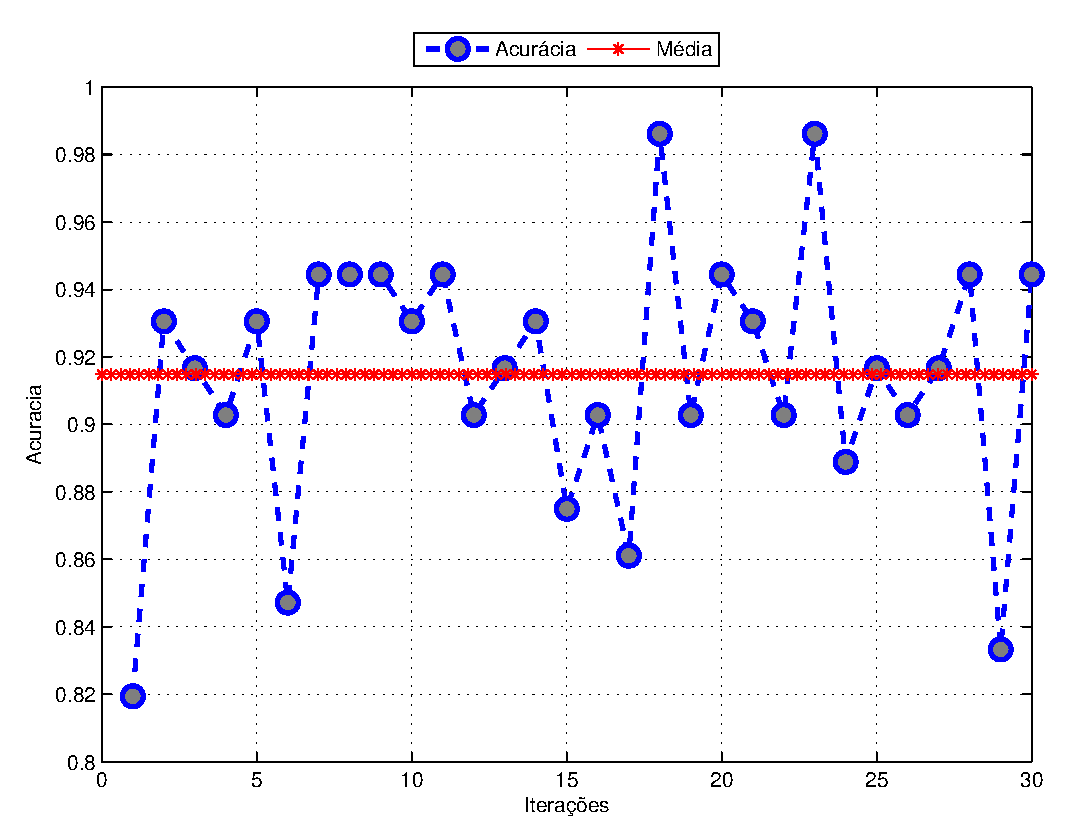
\includegraphics[width=0.4\textwidth]{figure/derme_parzen_h_1.eps}}
	\subfigure[h = 1,5]{ 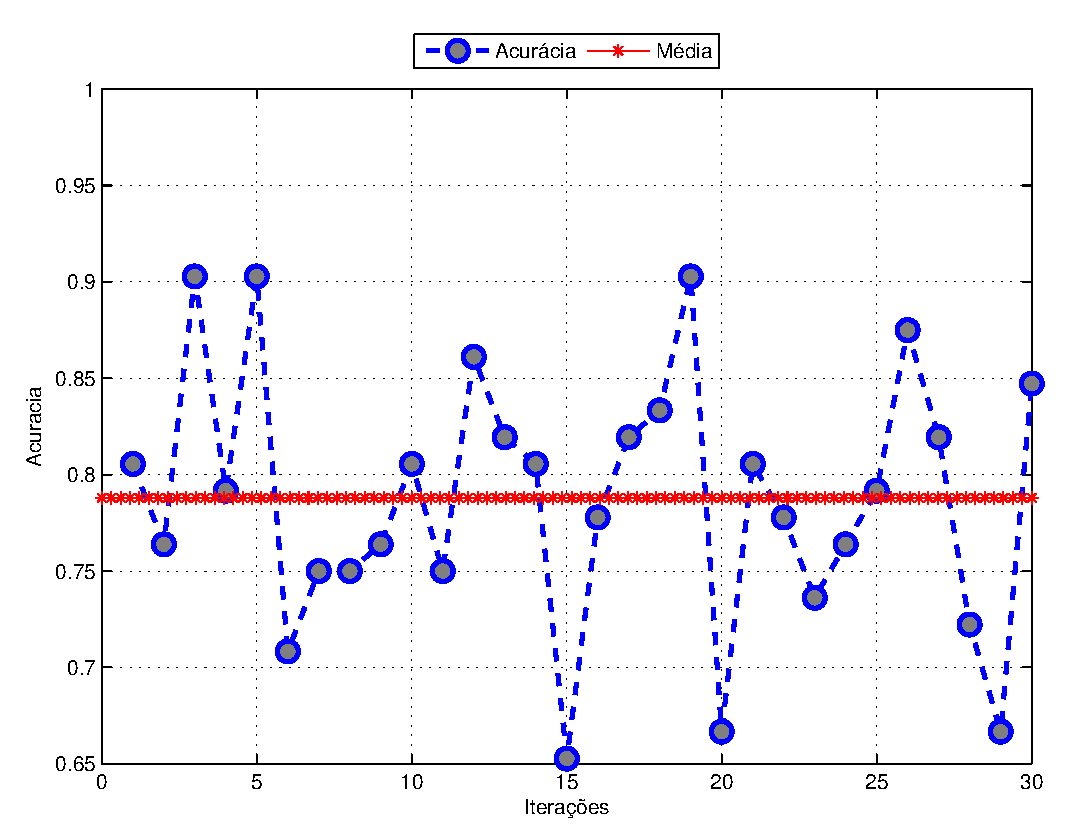
\includegraphics[width=0.4\textwidth]{figure/derme_parzen_h_15.eps}}
	\subfigure[h = 2]{ 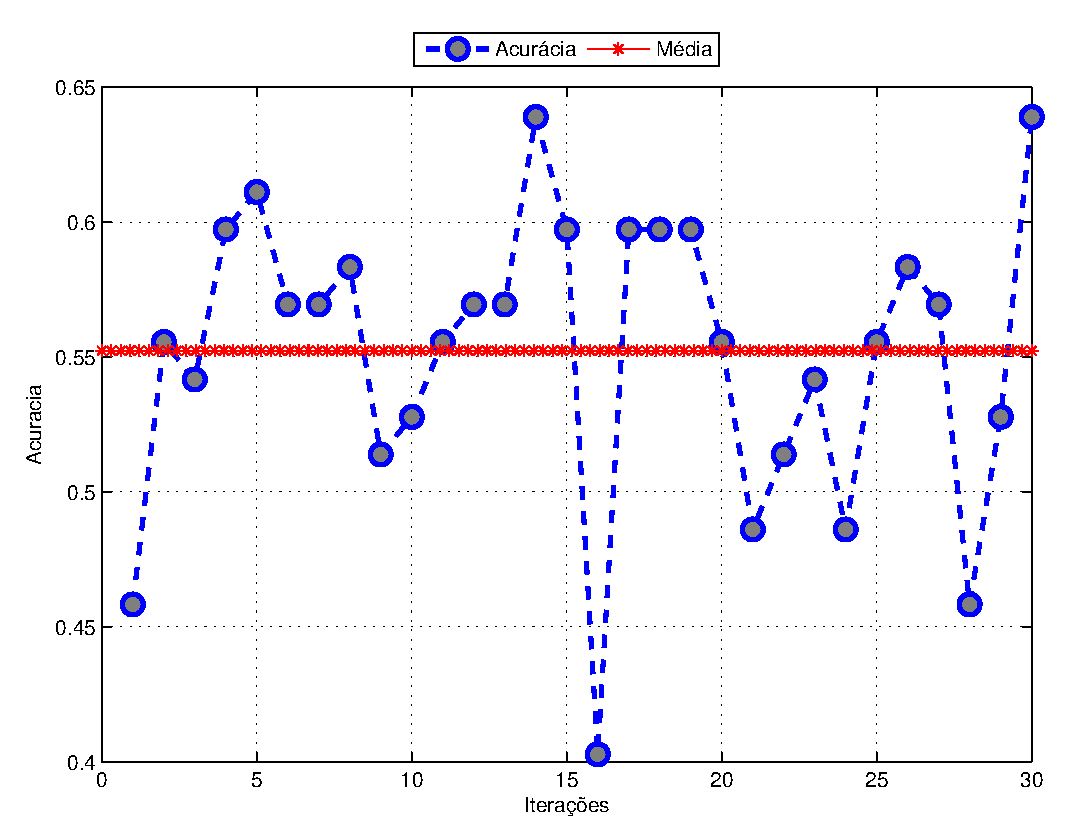
\includegraphics[width=0.4\textwidth]{figure/derme_parzen_h_2.eps}}
	
	\caption{Resultados da Acurácia para Derme.}
	\label{fig:accDerme}
\end{figure}


\subsection{Região de Decisão para Flor de Íris}

Em geral, um classificador particiona o espaço de características em volumes designados regiões de decisão. Todos os vetores de características no interior de uma região de decisão são atribuídos à mesma categoria.

O efeito de qualquer regra de decisão é dividir o espaço de características em c regiões de decisão R1, R2, $\cdots$, Rc . Se $g_i (x) > g_j(x)  \forall_j \neq i$, então x está em $R_i$.

As regiões são separadas por superfícies de decisão, isto é, as superfícies formadas pelos pontos que pertencem a mais de uma função discriminante (interseção entre as superfícies).

\begin{figure}[H]
	\centering
	
	\subfigure[]{ \includegraphics[width=0.3\textwidth]{figure/decisionboundary_12.eps}}
	\subfigure[]{ \includegraphics[width=0.3\textwidth]{figure/decisionboundary_13.eps}}
	\subfigure[]{ \includegraphics[width=0.3\textwidth]{figure/decisionboundary_14.eps}}
	\subfigure[]{ \includegraphics[width=0.3\textwidth]{figure/decisionboundary_23.eps}}
	\subfigure[]{ \includegraphics[width=0.3\textwidth]{figure/decisionboundary_24.eps}}
	\subfigure[]{ \includegraphics[width=0.3\textwidth]{figure/decisionboundary_34.eps}}
	
	\caption{Região de Decisão para flor da Íris.}
	\label{fig:decisionRegionIris}
\end{figure}

\section{Conclusões}

As técnicas de Aprendizagem de Máquina tem sido cada vez mais usadas para resolver todos os tipos de problemas da computação. São vários os motivos pelo seu uso, tendo destaque a sua maior flexibilidade, adaptabilidade e bons resultados gerado.

Neste relatório, foi apresentado e implementado o classificador de Parzen usado para segmentar imagens digitais e classificar dois tipos de bases, demonstrando que o aprendizado é uma abordagem bastante simples e robusta, com valores de acurácia bem satisfatório e minimizando as taxas de erro. 

%% The Appendices part is started with the command \appendix;
%% appendix sections are then done as normal sections
%% \appendix

%% \section{}
%% \label{}

%% References 
%%
%% Following citation commands can be used in the body text:
%% Usage of \cite is as follows:
%%   \cite{key}         ==>>  [#]
%%   \cite[chap. 2]{key} ==>> [#, chap. 2]
%%

%% References with bibTeX database:

\bibliographystyle{elsarticle-harv}
%\bibliographystyle{elsarticle-num}
%\bibliography{<your-bib-database>}

%% Authors are advised to submit their bibtex database files. They are
%% requested to list a bibtex style file in the manuscript if they do
%% not want to use elsarticle-num.bst.

%% References without bibTeX database:

\section*{Referências}

\begin{thebibliography}{01}

%% \bibitem must have the following form:
%%   \bibitem{key}...
%%

% \bibitem{}

\bibitem{DeGroot1989}
[DeGroot, 1989] DeGroot, M. H. (1989). Probability and Statistics. Addison-Wesley, 2nd edition.

\bibitem{Duda2001}
[Duda et al., 2001] Duda, R. O., Hart, P. E., and Stork, D. G. (2001). Pattern Classification. John Wiley and Sons.

\bibitem{Epanechnikov1969}
Epanechnikov, V.A. (1969). "Non-parametric estimation of a multivariate probability density". Theory of Probability and its Applications 14: 153–158.

\bibitem{Frutuoso2013}
Frutuoso, R. L. Identificação de Órgãos foliares utilizando as wavelets de daubechies. XIV Workshop de Informática Médica, FCT/UNESP, v. 1, n. 1, p. 211–126, 2013. ISSN none. Disponível em: <http://www.lbd.dcc.ufmg.br/colecoes/wvc/2010/0037.pdf>. Citado na página 8.

\bibitem{Kohavi1995}
Kohavi, R. A study of cross-validation and bootstrap for accuracy estimation and model selection. In: International joint Conference on artificial intelligence. [S.l.: s.n.], 1995. v. 14, p. 1137–1145.

\bibitem{Kohn1999}
[Kohn, 1999] Kohn, A. F. (1999). Reconhecimento de Padrões - Uma Abordagem Estatística. EPUSP.

\bibitem{Meyer1969}
[Meyer, 1969] Meyer, P. L. (1969). Probabilidade - Aplicações à Estaística. Ao Livro Técnico S.A. Versão traduzida do original em inglês.

\bibitem{Parzen1962}
Parzen, E. (1962). "On Estimation of a Probability Density Function and Mode". The Annals of Mathematical Statistics 33 (3): 1065.

\bibitem{Rosenblatt1956}
Rosenblatt, M. (1956). "Remarks on Some Nonparametric Estimates of a Density Function". The Annals of Mathematical Statistics 27 (3): 832.

\bibitem{Scaranti2010}
Scaranti, A. ; Bernardi, R. ; Plotze, R. O.. (2010) “Identificação de Órgãos Foliares Utilizando as Wavelets de Daubechies”. In: WVC'2010 - VI Workshop de Visão Computacional.

\bibitem{UCI152015}
[UCI15] Uci machine learning repository, 2015. Disponível em: <http:// archive.ics.uci.edu/ml/>.

\bibitem{Wand1995}
Wand, M.P; Jones, M.C. (1995). Kernel Smoothing. London: Chapman \& Hall/CRC. ISBN 0-412-55270-1.


\end{thebibliography}


\end{document}

%%
%% End of file `elsarticle-template-num.tex'.
